\section{Scene-Graph}
% \subsection{Multiple objects}\label{sec:multiple}
When the simulation involves several objects, we model them as different branches in a scenegraph data structure.
In the example shown in Figure~\ref{fig:twoObjects}, the scene contains two objects animated using different time integrators, collision detection components (discussed in Section~\ref{sec:collision}), an interaction force, and a camera to display the objects.
The root node does not contain DOFs.
It is used to contain the components which are common to its child nodes.
\begin{figure}
 \begin{center}
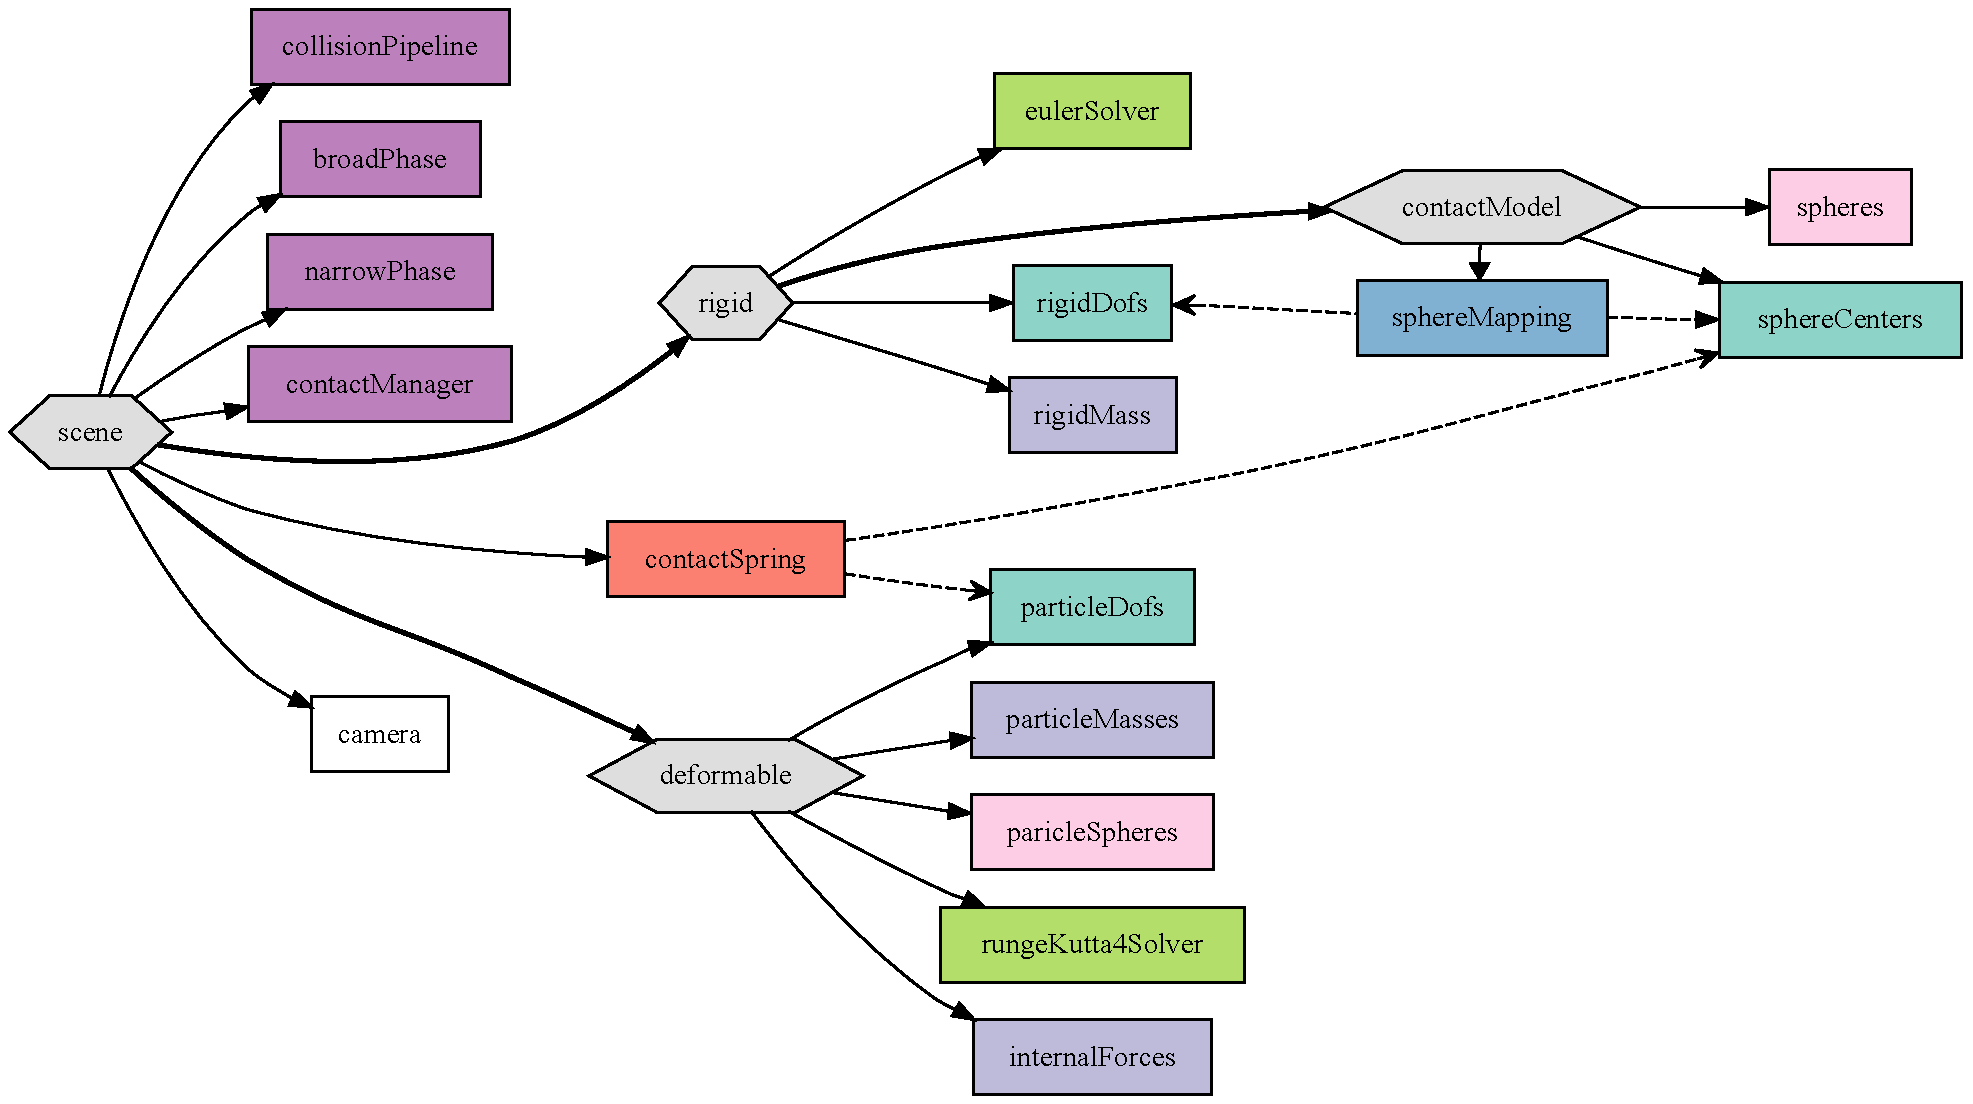
\includegraphics[width=0.98\linewidth]{twoObjects.pdf}
 \caption{A scenegraph with collision detection and two independent objects interacting through a spring.}                                                                      
 \label{fig:twoObjects}
\end{center}
\end{figure}
% Applying the same ODE solver to all the objects is as simple as attaching the corresponding component to the common ancestor node.
% This allows to process the objects and their interaction forces in a common equation system, which is necessary when stiff interaction forces or Lagrange multipliers are used for coupling the objects. 
% When each object has its own solver, the interaction force is considered constant during the time step.

Scenegraphs are popular in Computer Graphics due to their versatility.
The data structure is processed using visitors (discussed in Section~\ref{sec:visitors}) which apply virtual functions to each node they traverse, which in turn apply virtual functions to the components they contain.
% , and the visitor-based approach presented in Section~\ref{sec:visitors} allows us to apply operations to all the branches, possibly in parallel. 
In basic scenegraph frameworks, the visitors are exclusively fired from an external control structure such as the main loop of the application.
In \sofa, the components are allowed to suspend the current traversal to send an arbitrary number of other visitors, then to resume or to prune the suspended visitor.
This allows us to implement global algorithms (typically ODE solution or collision detection), such as the explicit Euler velocity update of Equation~\ref{eq:expliciteulerexample}, in components.
This neatly decouples the physical model from the simulation algorithms, in sharp contrast with dataflow graphs which intricate data and operators in the same graph.
Replacing a time integrator requires the replacement of one component in our scenegraph, whereas the corresponding dataflow graph would have to be completely rewritten.




Interactions between objects may be handled using penalty forces or Lagrange multipliers. 
In all cases, a component connected to the two objects is necessary to geometrically model the contact and compute the interaction forces.
This component being shared between the two objects, it is located in their common ancestor node.
The coupling created by penalty forces should be seen as soft or stiff, depending on the stiffness and the size of time step~\cite{baraff98large}.
A soft coupling can be modeled by an interaction force constant during each time step.
In this case, each object can be animated using its own, possibly different, ODE solver.
% The interaction force is computed and accumulated  when the AnimateVisitor traverses the ancestor nodes before reaching each solver in their child branches.
% This ensures that the object undergo opposite interaction forces during the time step, but it requires the synchronization of the object at the end of each time step.
% Animating the two objects at different time steps would be possible, using each solver independently instead of a common AnimateVisitor, but this would require an additional mechanism to update the interaction and enforce Newton's third law on opposite forces.
The assumption of constant interaction force during each time step is compatible with all explicit time integration methods.
However, when the interaction forces are stiff, implicit integration is necessary to apply large time steps without instabilities.
This requires the solution of an equation system involving the two objects as well as their interaction force together.
In this case, the ODE solver is placed in the common ancestor node, at the same level as the interaction component.
This is also true for constraint-based interaction which requires the computation of Lagrange multipliers based on interaction Jacobians. 
% \todo{illustrer sur une figure}
% We call it \textit{hard coupling} when the interacting objects and the interaction forces need to be solved simultaneously in a common equation system.
% This includes stiff penalty forces and Lagrange multipliers.
Due to the superlinear time complexity of equation solvers, it is generally more efficient to process independent interaction groups using separated solvers rather than a unique solver.

% 
% Contact interactions created during the simulation may be soft, stiff of constraint-based, depending on the collision response stategy, as explained in Section~\ref{sec:collision}.
% In case of hard coupling, a group manager is used to gather objects in the smallest possible groups.


% \subsubsection{The context} \label{sec:components}
% \SC{I would remove this subsection - it is redundant with some of the other text}
% 
% % \todo{Description plus détaillée des composants : principe de séparation des données (State,TopoContainer), des calculs (FF,TopoModifier,...), et des dépendances (Node)}
% % 
% % \todo{Présentation de l'utilisation des templates : comment ils permettent dans les composants d'avoir des codes génériques tout en étant instancié et optimisé par le compilateurs pour chaque type de DOF.}
% All the components acting on the same DOFs are gathered in a common node, which main contain: 
% % A node may represent a set of physical objects, such as the root of the scene or a collision group, using the list of child nodes.
% % Groups may contain algorithm components, applied to all the children using graph visitors as explained in Section~\ref{sec:visitors}. 
% % These include ODE solvers to integrate time, collision detection algorithms, and MasterSolvers to schedule the formers.
% % Groups may also include components associated with interactions between the child nodes, as discussed in Section~\ref{sec:interactions}.
% % A node may also represent one kinematic layer of a physical object, i.e. a set of components associated with the same degrees of freedom.
% % This includes: 
% \begin{itemize}
%  \item a container of state vectors, to represent coordinates, velocities, forces, accelerations and any auxiliary vector used by the algorithms. Each state vector contains the values associated to all the nodes. All the following components in this list read and write the state vectors in this component.
%  \item a list of topology containers, to model mesh edges, faces and cells based on node indices.
%  \item a mass, to compute accelerations based on forces, and momentums based on velocities.
%  \item a list of force functions, to accumulate forces based on positions and velocities. They can be used to model internal or external forces, including force boundary conditions.
%  \item a list of projective constraints, to filter the state vectors to cancel forbidden displacements. They can be used to apply displacement boundary conditions to each indendent DOF.
%  \item lists of geometrical primitives used in collision detection.
%  \item a list of child nodes, to create hierarchies and complex scenes (see sections~\ref{sec:mappings} and \ref{sec:scenes})
%  \item a mapping, to synchronize the local DOFs with master DOFs higher in the hierarchy
%  \item a list of constraints to handle using Lagrange multipliers, more complex but more general than projective constraints. They can be used to apply constraints to non-independent DOFs.
%  \item lists of components implementing algorithms for collision detection(\ref{sec:collision}) and the solution of equations (section~\ref{sec:odesolvers})
% \end{itemize}
% While most of the data is private, some is available to all the components, especially the topology and the state vectors. 
% % These attributes are used by the visitors to access the components during the graph traversals.
% % The connections between the components attached to the same node are generally implicit, because there is a unique container of state vector and a unique topology, which allows the components to find the necessary data.
% For instance, 
% % a TetrahedronFEMForceField computes viscoelastic forces based on the deformation of tetrahedra. 
% the list of tetrahedra used by a TetrahedralFEMForceField is stored in the local topology container, while the initial and current particle states are stored in the MechanicalObject. 
% The same list of tetrahedra may be used to define the embedding of auxiliary DOFs in children nodes, as discussed in Section~\ref{sec:mappings}.
% % Additionally, nodes contain lists of control components to implement simulation algorithms, such as EulerSolver, as discussed in Section~\ref{sec:control}.


